\documentclass[]{project_report}
\author{%
	Marcin Lembke\\
	\texttt{\href{mailto:M.Lembke@stud.elka.pw.edu.pl}%
			{\nolinkurl{M.Lembke@stud.elka.pw.edu.pl}}}
	\and
	Marcin Malesa\\
	\texttt{\href{mailto:M.Malesa@stud.elka.pw.edu.pl}%
			{\nolinkurl{M.Malesa@stud.elka.pw.edu.pl}}}
}
\supervisor{dr inż. Piotr Bilski}
\title{Algorytm przeszukiwania z tabu do rozwiązywania układanki Sudoku (PB5)}
\subtitle{Sprawozdanie wstępne}
\course{Współczesne metody heurystyczne}
\coursecode{WMH}
\university{Politechnika Warszawska}
\faculty{Wydział Elektroniki i Technik Informacyjnych}

\addbibresource{bibliography.bib}

\begin{document}
	\maketitle
	
	\section{Sudoku}
	Sudoku to gra logiczna, której celem jest uzupełnienie planszy, zazwyczaj o rozmiarze 9 na 9 pól, w taki sposób aby w każdym wierszu, kolumnie oraz wyznaczonym bloku 3 na 3 pola, znalazło się po jednej cyfrze z zakresu 1 do 9.
	
	\begin{figure}[H]
		\centering
		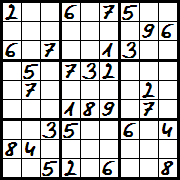
\includegraphics[scale=0.8]{sudoku_example.png}
		\caption{Przykładowa plansza Sudoku. Pogrubionymi liniami oznaczono bloki o rozmiarze 3 na 3 pola. Źródło: \href{https://upload.wikimedia.org/wikipedia/commons/2/2d/Sudoku_przyklad.png}{wikimedia.org}}
	\end{figure}
	
	\section{Przeszukiwanie tabu}
	Przeszukiwanie tabu (ang. \textit{Tabu search}, TS) to metaheurystyka wykorzystywania wraz z metodami przeszukiwania przy problemach optymalizacyjnych.
	
	Ideą algorytmu jest iteracyjne przeszukiwanie przestrzeni możliwych rozwiązań. Przy każdym ruchu korzysta się z tak zwanej listy tabu (ang. \textit{Tabu list}).
	
	Mając zadane rozwiązanie \(x\) przeszukiwane jest jego sąsiedztwo w celu w celu uzyskania rozwiązania \(x'\). Każde rozwiązanie jest oceniane według zadanej funkcji oceny (nazywanej także funkcją celu). Problemem takiego przeszukiwania jest możliwość zatrzymania się algorytmu w minimum lokalnym.
	
	W celu wykluczenia takich sytuacji wykorzystywana jest właśnie lista tabu, która zawiera ruchy niedozwolone (np. wykonane ostatnio).
	
	\section{Podstawowe problemy i ich wstępne rozwiązania}
	Analizując zadanie zaprojektowania i implementacji algorytmu do rozwiązywania łamigłówki Sudoku wykorzystującego przeszukiwanie tabu można dostrzec pewne podstawowe problemy:
	
	\begin{enumerate}
		\item Jak generować plansze do testowania -- liczba możliwych (rozwiązanych) plansz to ponad \(6,67 \cdot 10^{21}\)\cite{OEIS}. Ponadto liczba plansz dających się jednoznacznie rozwiązać wynosi ponad 49 tys. dla 17 uzupełnionych pól.
		
		Problem można przedstawić następująco: w jaki sposób wygenerować planszę do Sudoku dającą się jednoznacznie rozwiązać i jak generować planszę o zadanym stopniu trudności.
		
		Jeśli chodzi o generowanie jednoznacznie rozwiązywalnych plansz to pierwszym co przychodzi na myśl jest stworzenie bazy ,,dobrych'' plansz, na podstawie których będą generowane następne plansze. Pomysł jest dość prymitywny i jest obciążony dodatkowym problemem jakie przekształcenia wykonywać, aby wciąż utrzymać jednoznaczność rozwiązania.
		
		Drugim pomysłem jest wykorzystanie sposobu zaproponowanego w \cite{McGuire2013}. Główną ideą przedstawionego rozwiązania problemu jest wygenerowanie planszy rozwiązanej wykorzystując algorytm z rodziny ,,Las Vegas'', a następnie usunięciu niektórych pól. Algorytm rozwiązuje też zagadnienie trudności planszy -- usuwa się liczę uzupełnionych pól w zależności od stopnia trudności.
				
		\item Jak zdefiniować sąsiedztwo -- algorytm przeszukiwania tabu wymaga od nas zdefiniowania relacji sąsiedztwa na parach elementów przestrzeni rozwiązań, która będzie obejmować jej całą dziedzinę.  W przypadku Sudoku, może to po  prostu być funkcja swap(i, j), która zamienia ze sobą elementy z pozycji i-tej oraz j-tej w danym bloku.
		
		\item Jak reprezentować listę tabu -- listę tabu można reprezentować jako kolejkę FIFO (ang. \textit{First In, First Out}) o zadanym rozmiarze, w której w przypadku przekroczenia zadanego rozmiaru kolejki usuwane są najstarsze elementy.
		
		\item Określenie pamięci długoterminowej -- przeszukiwanie tabu wykorzystuje pamięć długoterminową do przechowywania najlepszego globalnie rozwiązania, które zostaje zwrócone na końcu algorytmu. Może to być pojedyncze rozwiązanie bądź lista najlepszych rozwiązań.
		
		\item Kryterium aspiracji -- jeśli zostanie spełnione, umożliwia wykonanie ruchu znajdującego się na liście tabu. Może to być np. próg wartości funkcji oceny. Jeśli ruch z listy tabu powoduje, że rozwiązanie jest lepsze od najlepszego o wartość tego progu, to ruch ten będzie akceptowalny.
		
	\end{enumerate}
	
	\printbibliography
\end{document}
